\documentclass[compress]{beamer}
\usepackage[utf8]{inputenc}
\usepackage{hyperref}

\usepackage{tikz}
\usetikzlibrary{graphs, quotes, arrows.meta, matrix}

\usetheme{default}
\usecolortheme{Nord}
\setbeamertemplate{navigation symbols}{}

\title{Tecniche avanzate su alberi}
\subtitle{Linearizzazione e Small to Large}
\author{Lorenzo Ferrari, Davide Bartoli}
\date{\today}

\begin{document}

\begin{frame}
    \maketitle
\end{frame}

\begin{frame}{Table of contents}
  \tableofcontents
\end{frame}

\section{Linearizzazione di un albero}
\begin{frame}{Problema motivazionale}{Subtree queries}
    \begin{exampleblock}{Subtree queries}
        \`E dato un albero radicato in $1$ con $N \leq 100'000$ nodi. Ogni nodo ha un valore. Performa $Q$ di queste operazioni:
        \begin{enumerate}
            \item cambia il valore del nodo $s$ a $x$
            \item calcola la somma dei valori nel subtree del nodo $s$
        \end{enumerate}
    \small{\underline{\url{https://cses.fi/problemset/task/1137}}}
    \end{exampleblock}
    Come si risolve un problema del genere?
    \begin{itemize}
        \item un'idea \`e fare update in $O(1)$ e query in $O(N)$ con una dfs
        \pause
        \item un'alernativa \`e fare update in $O(N)$ e query in $O(1)$
        \pause
        \item la complessit\`a di entrambe le soluzioni \`e $O(N Q)$
    \end{itemize}
        \pause
    Si pu\`o fare meglio di cos\`i?
\end{frame}

\begin{frame}{Ordine DFS}
    Facciamo una \textbf{DFS} sull'albero, per ogni nodo salviamo:
    \begin{itemize}
        \item il tempo \texttt{tin[v]} in cui la dfs entra nel nodo \texttt{v}
        \item il tempo \texttt{tout[v]} in cui la dfs esce dal nodo \texttt{v}
    \end{itemize}
    \pause
    Per come funziona la dfs, per ogni nodo \texttt{u} nel sottoalbero di \texttt{v} vale
    $$tin[v] < tin[u] < tout[u] < tout[v]$$
    \begin{block}{subtree = subarray}
        Nell'\textbf{ordine DFS}, i nodi in un subtree formano un subarray!
    \end{block}
    \pause
    Possiamo lavorare sui subtree come se lavorassimo su subarray dell'ordine dfs e usare le strutture dati che conosciamo per processare query e update efficientemente.
\end{frame}

\begin{frame}{Ordine DFS}
    \makebox[\textwidth]{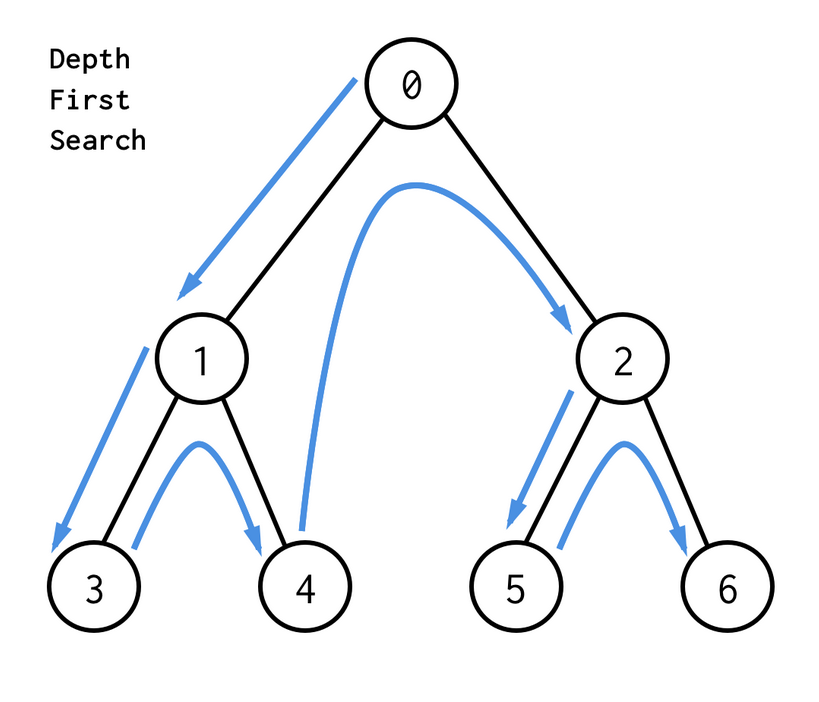
\includegraphics[scale=.28]{./img/dfs.png}}
    \begin{center}
    \tiny{http://mishadoff.com/blog/dfs-on-binary-tree-array/}
    \end{center}
\end{frame}

\begin{frame}{Altre applicazioni}{Ancestors query}
    \begin{block}{range update/point query}
        \begin{itemize}
            \item su un segment, potevamo passare facilmente da point update/range query a range update/point query
            \item la stessa idea si pu\`o usare su un albero linearizzato
        \end{itemize}
    \end{block}
    \pause
    \begin{exampleblock}{Path queries}
        \`E dato un albero radicato in $1$ con $N \leq 100'000$ nodi. Ogni nodo ha un valore. Performa $Q$ di queste operazioni:
        \begin{enumerate}
            \item cambia il valore del nodo $s$ a $x$
            \item calcola la somma dei valori sul percorso dal nodo $s$ alla radice
        \end{enumerate}
    \small{\underline{\url{https://cses.fi/problemset/task/1137}}}
    \end{exampleblock}
\end{frame}

\section{Small to large}
\begin{frame}{Problema motivazionale}{Distinct Colors}
    \begin{exampleblock}{Distinct Colors}
        Dato un albero radicato in $1$ con $N \leq 200'000$ nodi. Ogni nodo ha un colore. Per ogni nodo vogliamo 
        calcolare il numero di colori distinti nel suo sottoalbero.
    \small{\underline{\url{https://cses.fi/problemset/task/1139}}}
    \end{exampleblock}
    Potremmo pensare di linearizzare l'albero come abbiamo visto prima, in questo modo dobbiamo fare $N$ query, e 
    una query ci chiede quanti colori distinti ci sono in un intervallo.
    \pause
    Come facciamo a risolvere questo problema? Non è ovvio, ma possiamo risolverlo utilizzando un segment tree.
    \small{\underline{\url{https://cses.fi/problemset/task/1139}}}
\end{frame}

\begin{frame}{Problema motivazionale}{Distinct Colors}
    Questo problema è su un albero, possiamo quindi sfruttare questa proprietà per risolverlo in modo più semplice.\\
    \pause
    Proviamo a risolvere il problema facendo una singola dfs sul nostro albero, per ora senza preoccuparci della complessit\`a.
    \pause
    \makebox[\textwidth]{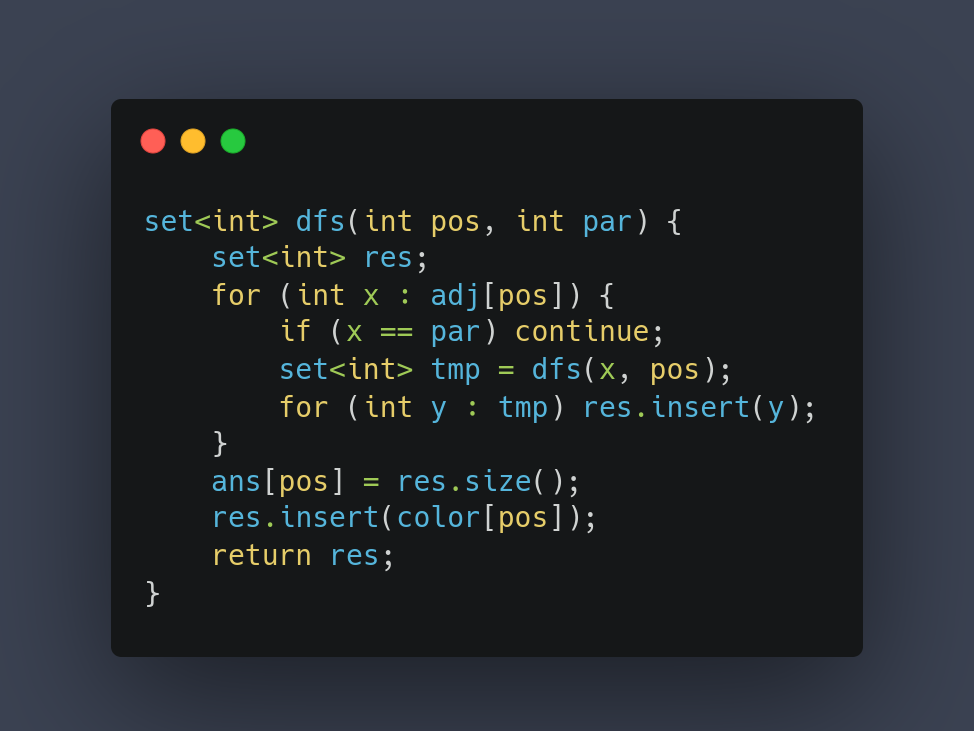
\includegraphics[scale=.27]{./img/dfs_no_s_to_l.png}}
\end{frame}

\begin{frame}{Problema motivazionale}{Distinct Colors}
    Qual \`e la complessit\`a di questa soluzione? $O(N^2)$, dato che unire due set ci richiede $O(N)$.\\
    \pause
    Possiamo modificare leggermente questa soluzione per renderla più veloce?\\
    \pause
    La risposta \`e s\`i, possiamo utilizzare la tecnica chiamata \textbf{small to large}.
    In particolare quando uniamo due set, possiamo mettere il set più piccolo dentro al set più grande.\\
    \pause
    Ma è più veloce? Si, infatti consideriamo un singolo elemento:\\
    ogni volta che viene spostato, si trova in un set grande almeno il doppio di quello in cui era prima.\\
    \pause
    Quindi viene spostato al massimo $O(\log N)$ volte, e la complessità totale è $O(N \log N)$.
\end{frame}

\begin{frame}{Problema motivazionale}{Distinct Colors}
    Dobbiamo però fare attenzione a come passiamo/ritorniamo il set dalle funzioni, in quanto non vogliamo che venga copiato (altrimenti la complessità cambia).
    \makebox[\textwidth]{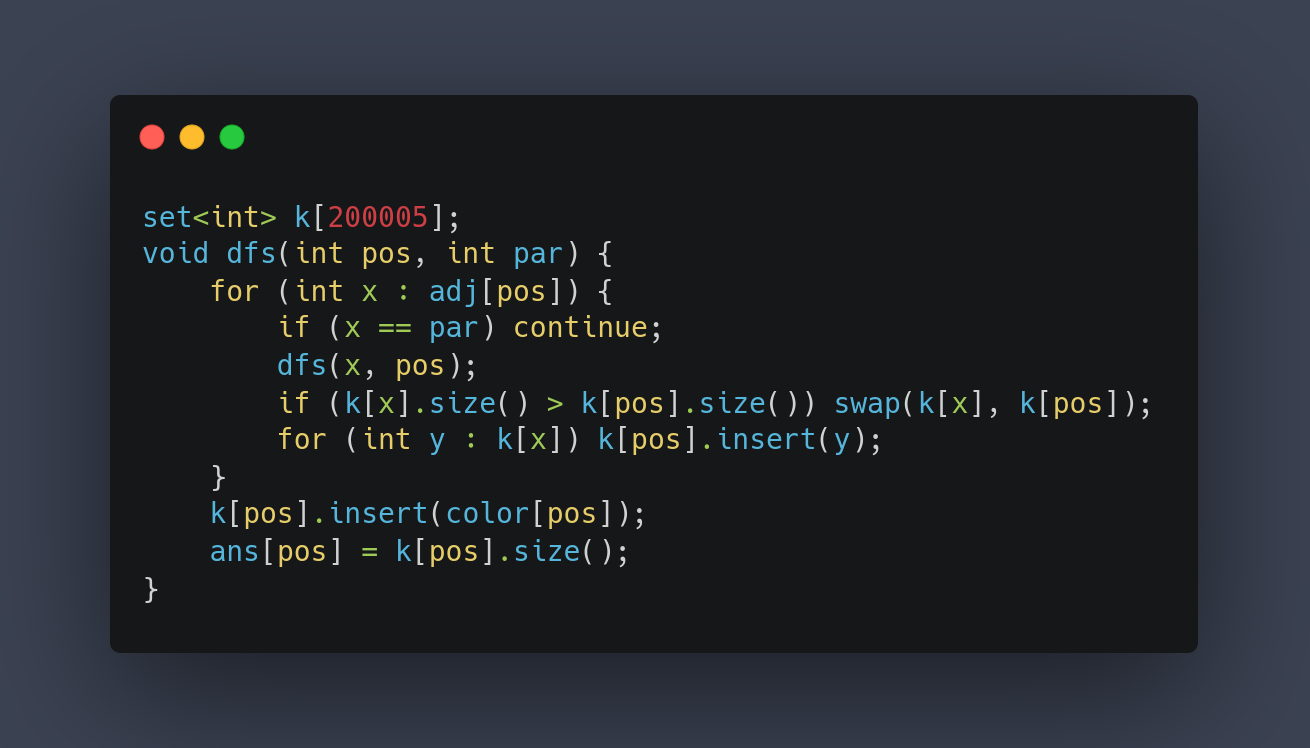
\includegraphics[scale=.27]{./img/dfs_s_to_l.png}}
\end{frame}

\section{Problemi}
\begin{frame}{Problemi}{(belli)}
    \small{\underline{\url{https://cses.fi/problemset/task/1137}}}
    \small{\underline{\url{https://cses.fi/problemset/task/1138}}}
    \small{\underline{\url{https://cses.fi/problemset/task/1139}}}
    \small{\underline{\url{https://training.olinfo.it/\#/task/ois_christmasballs/statement}}}
    \small{\underline{\url{https://training.olinfo.it/\#/task/ois_forum/statement}}}
    \small{\underline{\url{https://training.olinfo.it/\#/task/ois_fossils/statement}}}
\end{frame}

\end{document}
